\section{Alloy}
In this section will be provided a formal model of the problem achieved using Alloy.The model represent only the most important part of the problem, few things have been simplified leaving the more relevant constraints.\newline
For the sake of readability the generated world is split into three sub-worlds which will be explained below.

\subsection{Code}
\begin{lstlisting}[language=alloy]
open util/integer
---------------------------------
-- Enumerations
---------------------------------
sig Seed{}
sig Fertilizer{}
sig Forecast{}
sig District{}
sig Mandala{}
sig TypeOfProduction{}


---------------------------------
-- Typedef
---------------------------------
abstract sig Boolean{}
one sig TRUE extends Boolean{}
one sig FALSE extends Boolean{}

---------------------------------
-- Classes
---------------------------------
abstract sig Users{
	//username: one String
	//password: one String
}

sig Zone{
	mandala: one Mandala,
	district: one District
}

sig Location{
	zone: one Zone
	//address: one String
}

sig WeatherRequest{
	zone: one Zone,
	forecast: one Forecast
	//startDate: one Date
	//endDate: one Date
}

one sig Weather{
	weatherRequest: set WeatherRequest
}

sig TPM extends Users{}

sig Farmer extends Users{
	location: one Location,
	resilient: one Boolean
}

sig Report{
	//body: one String
}

one sig VisualizeInitiatives{
	reports: set Report
}

sig Event{
	farmer: one Farmer,
	//title: one String
	visited: one Boolean, 
	report: lone Report
}
	
sig DailyPlan{
	visit: set Event,
	//date: one Date
	confirm: one Boolean
}

sig Agenda{
	dailyPlan: set DailyPlan
}

sig Agronomist extends Users{
	zone: one Zone,
	agenda: one Agenda
}

sig SeedType{
	name: one Seed,
	kgSeed: one Int //float
}

sig FertilizerType{
	name: one Fertilizer,
	kgFertilizer: one Int //float
}

sig DataCultivation{
	crop: one SeedType,
	fertilizer: one FertilizerType,
	typeOfProduction: one TypeOfProduction,
	tonsPerAcre: one Int //float
}

sig DataProduction{
	farmer: one Farmer,
	waterUsed: one Int, //float
	soilHumidity: one Int, //float
	cultivations: some DataCultivation
}

one sig ReportProduction{
	dataProductions: set DataProduction
}

sig Problem{
	farmer: one Farmer
	//title: one String
	//problem: one String
}

one sig ReportProblem{
	problems: set Problem
}

sig Replies{
	farmer: lone Farmer,
	agronomist: lone Agronomist
	//reply: one String
}

sig HelpRequest{
	author: one Farmer,
	replies: set Replies
	//description: one String
}

one sig Help{
	helpRequest: set HelpRequest
}

sig DiscussionReplies{
	farmer: one Farmer
	//text: one String
}

sig Discussion{
	farmer: one Farmer,
	discussionReplies: set DiscussionReplies
	//title: one String
	//body: one String
}

one sig Forum{
	discussions: set Discussion
}

sig Messages{
	sender: one Users,
	receiver: one Users
	//body: one String
}

sig Chat{
	messages: set Messages
}

sig RankingType{
	farmer: one Farmer,
	performance: one Int
}

one sig Ranking{
	ranking: set RankingType
}

sig WikiFarmRequest{
	zone: one Zone,
	typeOfProduction: one TypeOfProduction
}

one sig WikiFarm{
	wikiFarmRequest: set WikiFarmRequest
}


---------------------------------
-- Facts
---------------------------------
-- Famers
fact Location{
	all l: Location | no disj f1, f2 : Farmer | f1.location = f2.location && 
	f1.location = l
}

fact ReportAllProblems {	
	all p: Problem | p in ReportProblem.problems
}

fact AllFarmerInRankingType{
	all f: Farmer | one r: RankingType | f in r.farmer
}

fact Ranking{
	all rt: RankingType | one r: Ranking | rt in r.ranking
}

fact NumberRankingType{
	(no p: RankingType.performance | p> #Ranking.ranking || p<=0) &&
	(no disj r1, r2: RankingType | r1.performance = r2.performance)
}

fact DataProduction{
	all d: DataProduction | (one f: Farmer | f in d.farmer) && (d.waterUsed >= 0) &&
	(d.soilHumidity >= 0)
}

fact DataCultivation{
	all d: DataCultivation | (one dp: DataProduction | d in dp.cultivations) &&
	(d.tonsPerAcre >= 0)
}

fact ReportProduction{
	all d: DataProduction | one r: ReportProduction | d in r.dataProductions
}

fact SeedTypeFertilizerType{
	(all s: SeedType | (one d: DataCultivation | s in d.crop) && s.kgSeed >= 0) &&
	(all f: FertilizerType | (one d: DataCultivation | f in d.fertilizer) && 
	f.kgFertilizer >= 0)
}

fact MandalaDistrict{
	all m: Mandala | one z: Zone | (m in z.mandala ) && (no z2: Zone | z != z2 && m in z2.mandala)
}

fact Replies{
	all r: Replies | (one h: HelpRequest | r in h.replies) && (#r.farmer != #r.agronomist) 
}

fact HelpRequest{
	all hr: HelpRequest | one h: Help | hr in h.helpRequest
}

fact DiscussionReplies{
	all dr: DiscussionReplies | one d: Discussion | dr in d.discussionReplies &&
	(no d2: Discussion | dr in d2.discussionReplies && d != d2 )
}

fact 	Discussion{
	all d: Discussion | (one f: Farmer | f in d.farmer) && (one f: Forum | d in f.discussions)
}

--Agronomist
fact OneAgendaForAgronomist{
	all a: Agenda | one ag: Agronomist | a in ag.agenda
} 

fact DailyPlan{
	all d: DailyPlan | one a: Agenda | d in a.dailyPlan
}

fact Event{
	(all e: Event | (one d: DailyPlan | e in d.visit) && (#e.report <= #e.visited) &&
	(#e.report = 0 => e.visited = FALSE else e.visited = TRUE)) 
}

fact Report{
	all r: Report | one e: Event | r in e.report
}

fact NoFarmerRepetitionEvent{
	all d: DailyPlan | no disj e , e2: Event | (e in d.visit && e2 in d.visit &&
	e.farmer = e2.farmer)   
}

fact SameZone{
	all e: Event | (one a:Agronomist, d: DailyPlan | d in a.agenda.dailyPlan && 
	e in d.visit && e.farmer.location.zone = a.zone)
}

fact VisualizeInitiatives{
	all r: Report | r in VisualizeInitiatives.reports
}

--Users
fact Messages{
	all m: Messages | (one c: Chat | m in c.messages) && (m.sender != m.receiver)
}

--System
fact Weather{
	all wr: WeatherRequest | one w: Weather | wr in w.weatherRequest	
}

fact WeatherRequest{
	all z: Zone | one w: WeatherRequest | z = w.zone
}

fact WikiFarmRequest{
	all wr: WikiFarmRequest | one w: WikiFarm | wr in w.wikiFarmRequest
}
\end{lstlisting}

\newpage
\subsection{Description of a general situation in Telangana}
The model highlights the case where there are 2 agronomists, agronomist0 and agronomist1, working in the same area.  Agronomist0 has two daily plans, the first one is confirmed, despite not meeting the original plan, while the second plan is unconfirmed, but the visit has taken place, this models the fact that the working day is not yet over. Agromist1 has a confirmed daily plan because he confirmed his visit to Farmer2 and has finished his working day.  Finally, Farmer0 is both resilient and first in Ranking, so he is qualified to receive incentives from Telangana.\\
Below is presented the code used for generating the model.
\begin{lstlisting}[language=alloy]
pred generalModel{
  #Seed = 0
  #Fertilizer = 0
  #TypeOfProduction = 0
  #DailyPlan = 3
  #Event = 4
  #DataProduction = 0
  #Forecast = 1
  #District = 1
  #Mandala >= #District
  #Zone = 2
  #Farmer = 3
  #TPM = 0
  #Agronomist = 2
  #HelpRequest = 0
  #Discussion = 0
}
run generalModel for 15
\end{lstlisting}
\begin{figure}[H]
\centering
	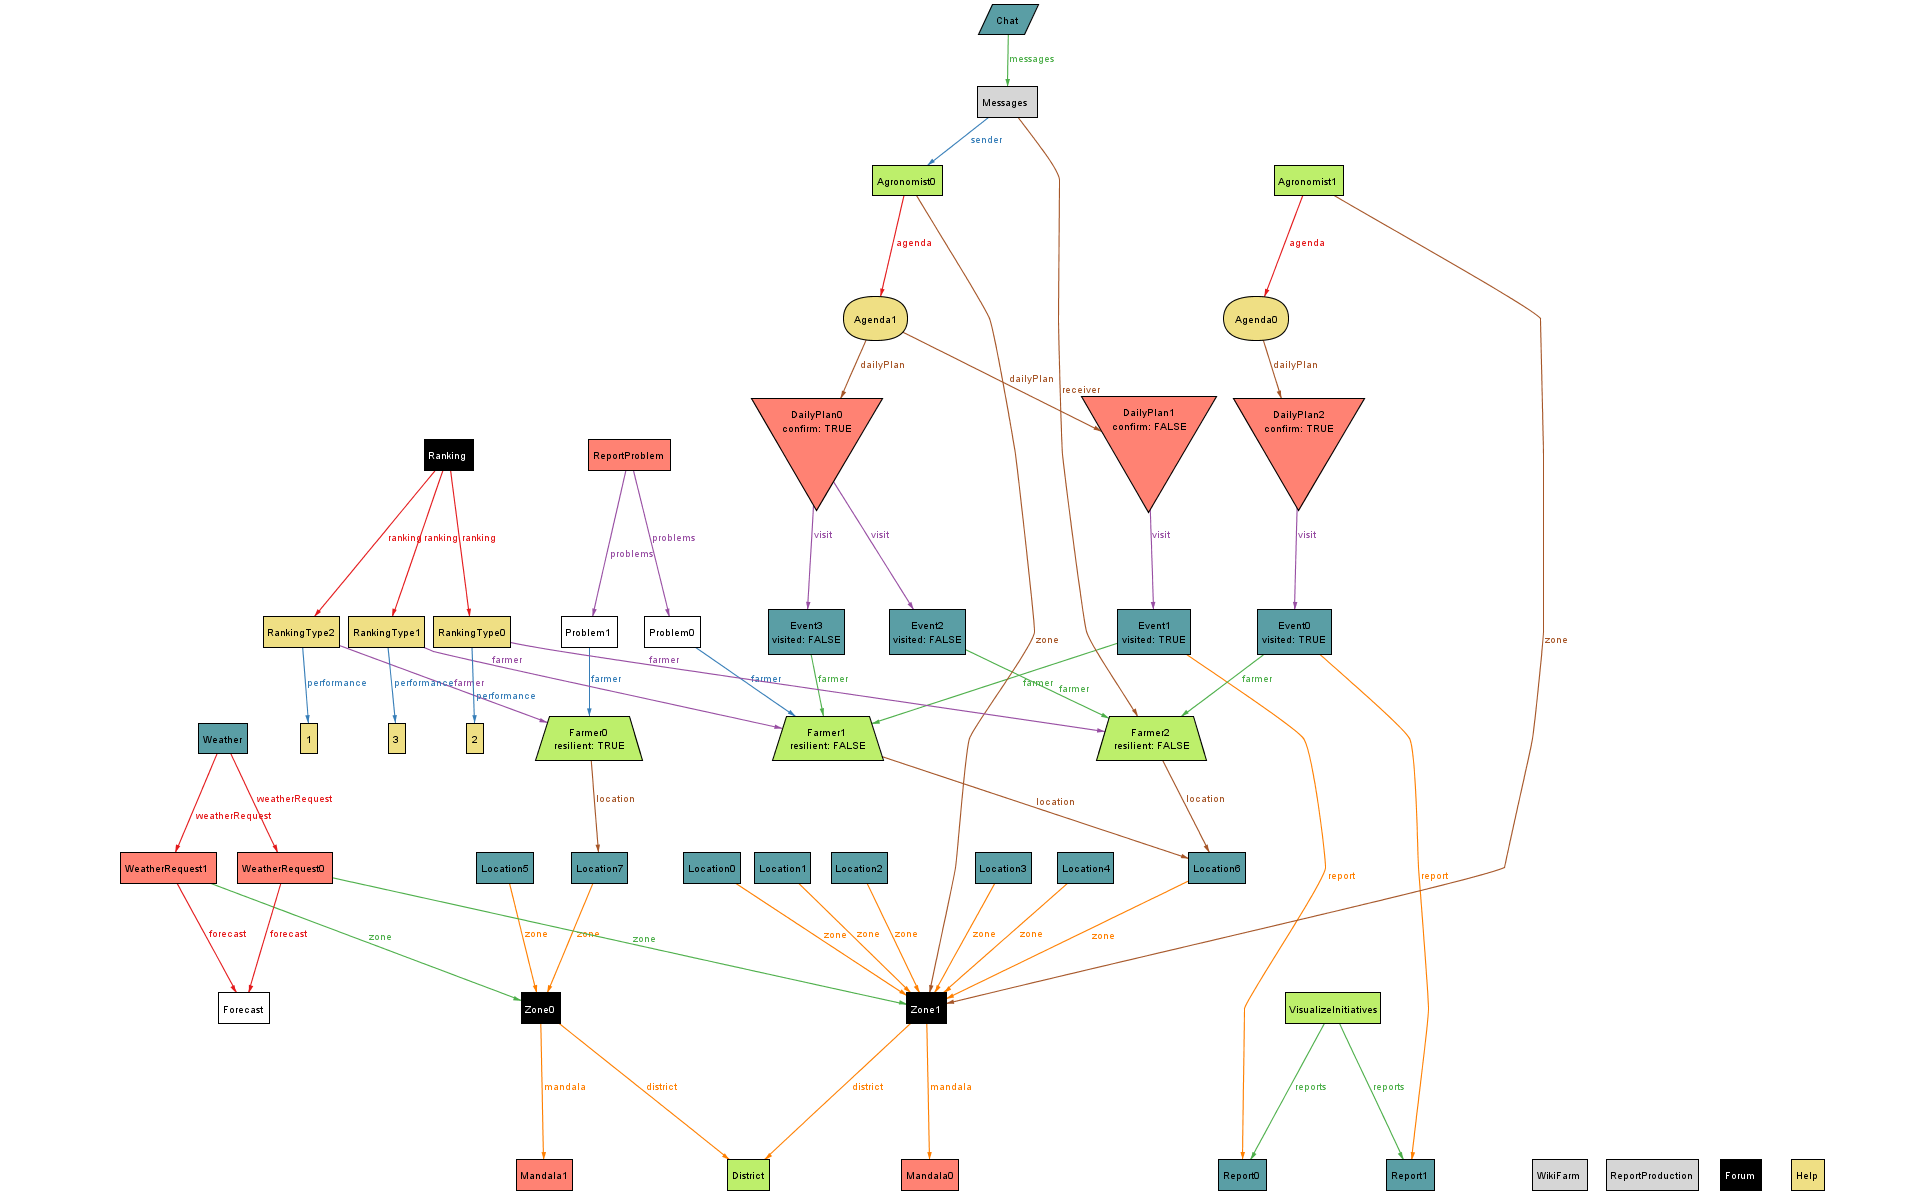
\includegraphics[angle=90,height=1.5\textwidth]{Images/Model/model1.png}
	\caption{Model of a general situation in Telangana}
\end{figure}
\subsection{Help Requests}
This graph represents two farmers requesting help. HelpRequest2 has a response from a farmer, while HelpRequest3 has a response from an agronomist. Both farmers also report a problem they have faced, using the ReportProblem function. In addition, both farmers present their DataProduction, Farmer1 presents two as one describes the most recent production, while the second represents a past situation.\\
Below is presented the code used for generating the model.
\begin{lstlisting}[language=alloy]
pred helpRequests{
  #DailyPlan = 0
  #DataProduction = 3
  #Forecast = 1
  #District = 1
  #Mandala >= #District
  #Zone = 1
  #Location = 2
  #Farmer = 2
  #TPM = 1
  #Agronomist = 1
  #HelpRequest = 4
  #Discussion = 0
  #WikiFarmRequest = 0
  #Replies.agronomist >= 1
  #Replies.farmer >= 1
}
run helpRequest for 15
\end{lstlisting}
\begin{figure}[H]
\centering
	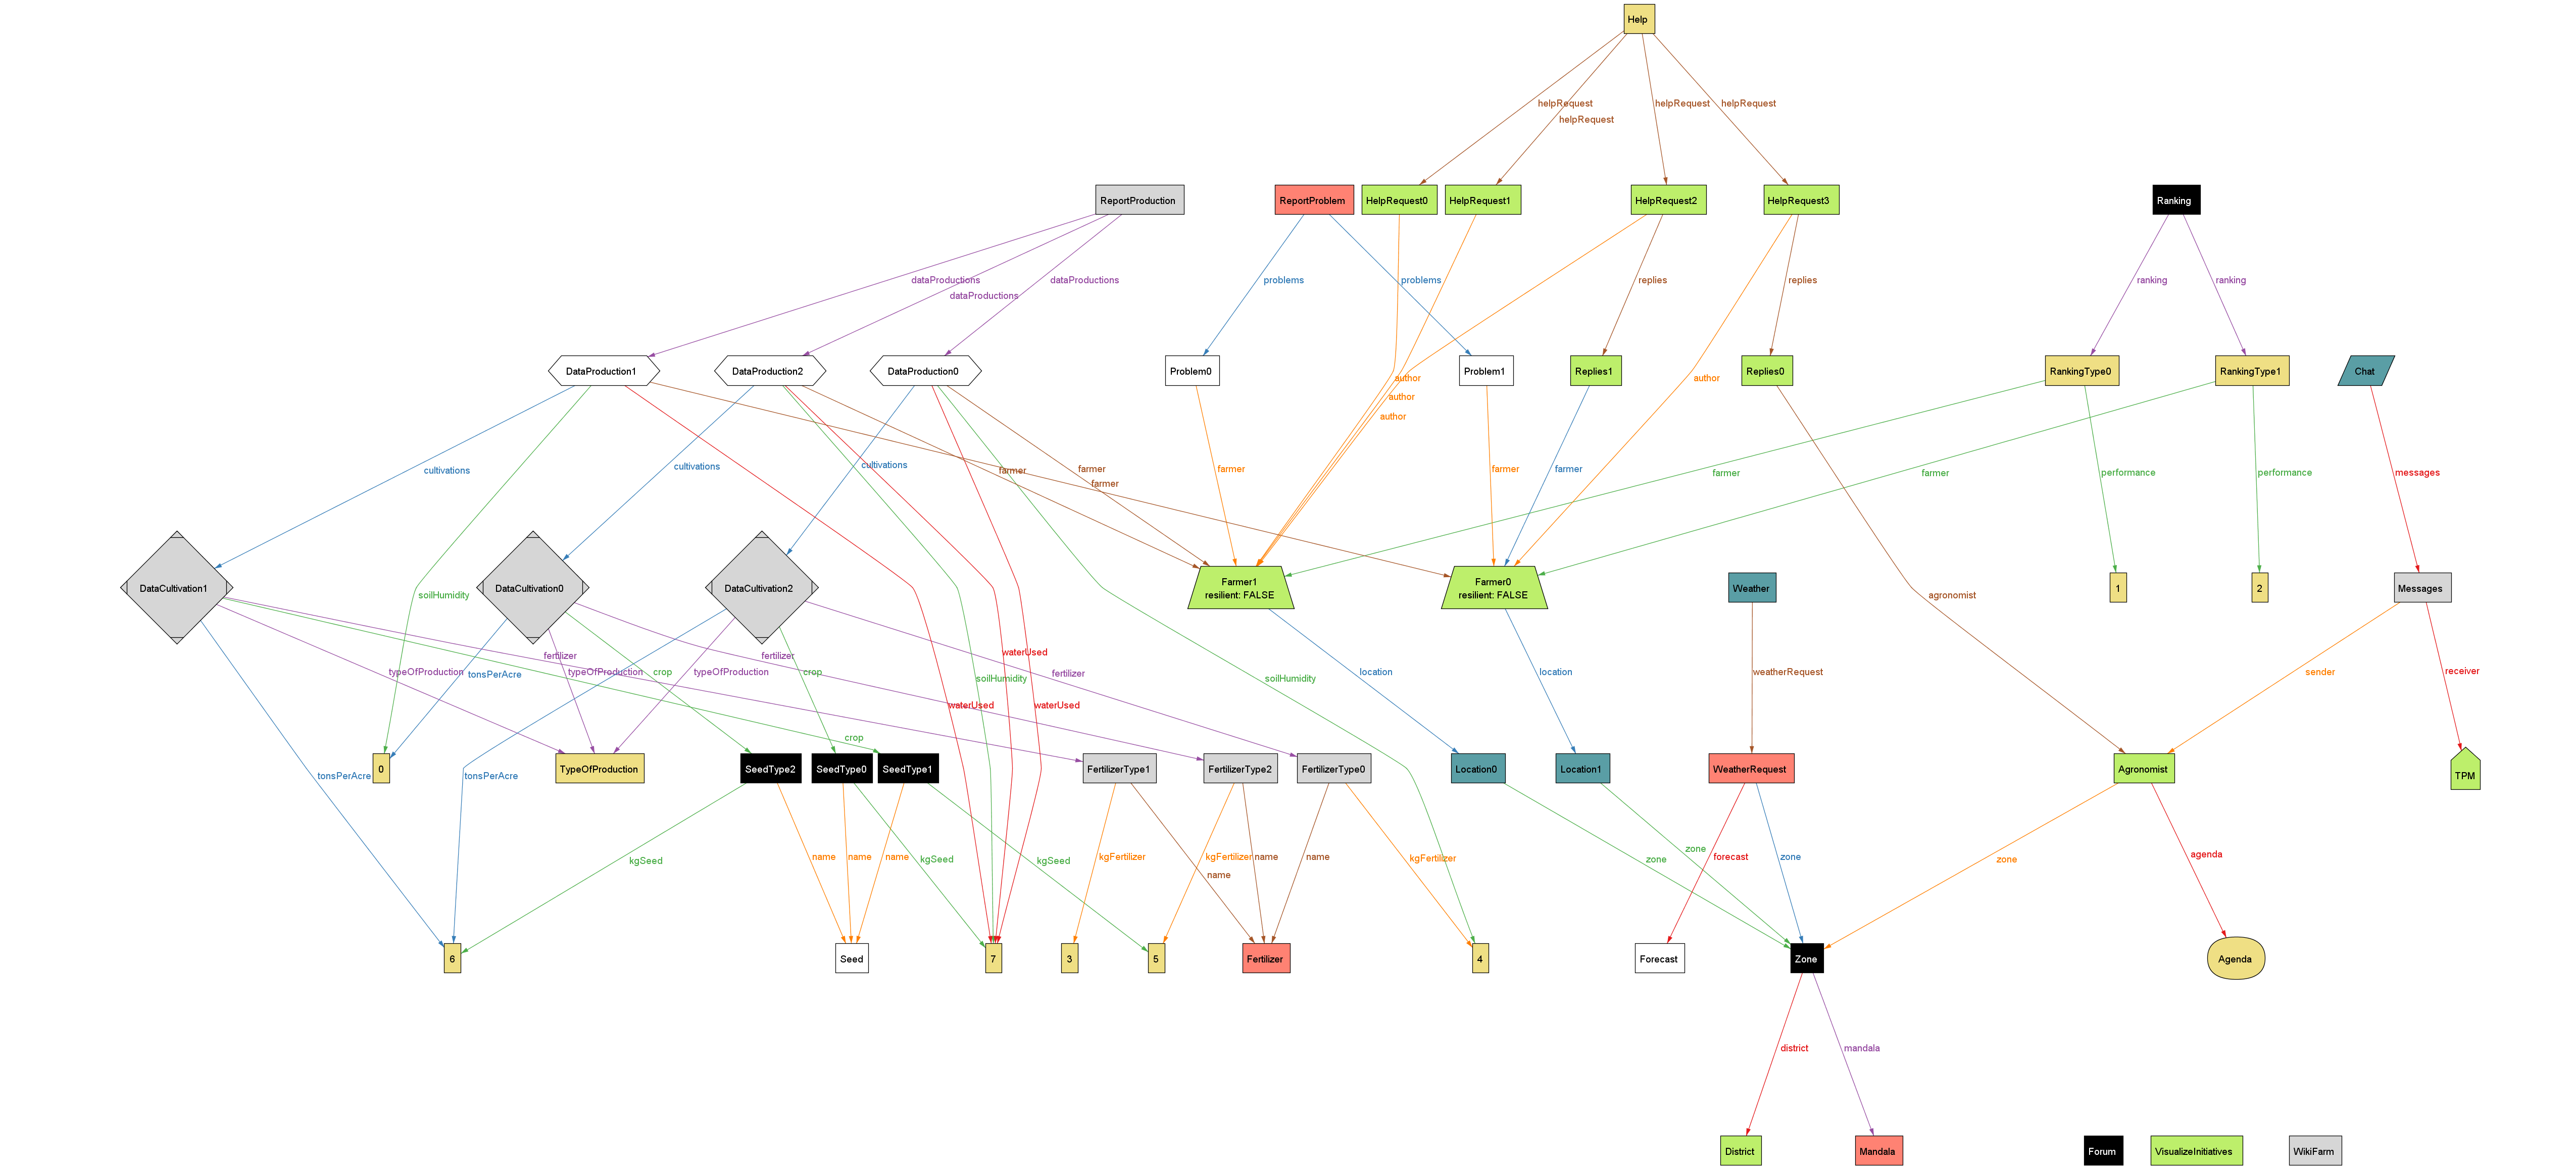
\includegraphics[angle=90,height=1.5\textwidth]{Images/Model/model2.png}
	\caption{Model of Help requests}
\end{figure}

\subsection{Discussions}
This graph shows that a farmer can create a Discussion in the Forum. Any farmer, even the creator, can also reply to the discussions. The most significant Discussion is Discussion5, which has replies from every farmer.\\
Below is presented the code used for generating the model.
\begin{lstlisting}
pred discussion{
  #Seed = 0
  #Fertilizer = 0
  #TypeOfProduction = 0
  #DailyPlan = 0
  #DataProduction = 0
  #Forecast = 1
  #District = 1
  #Mandala >= #District
  #Zone = 1
  #Farmer = 3
  #TPM = 0
  #Agronomist = 0
  #HelpRequest = 0
  #Discussion = 6
  #DiscussionReplies = 7
  #Problem = 0
  #Messages = 0
  #Location < 5
}
run discussion for 15
\end{lstlisting}
\begin{figure}[H]
\centering
	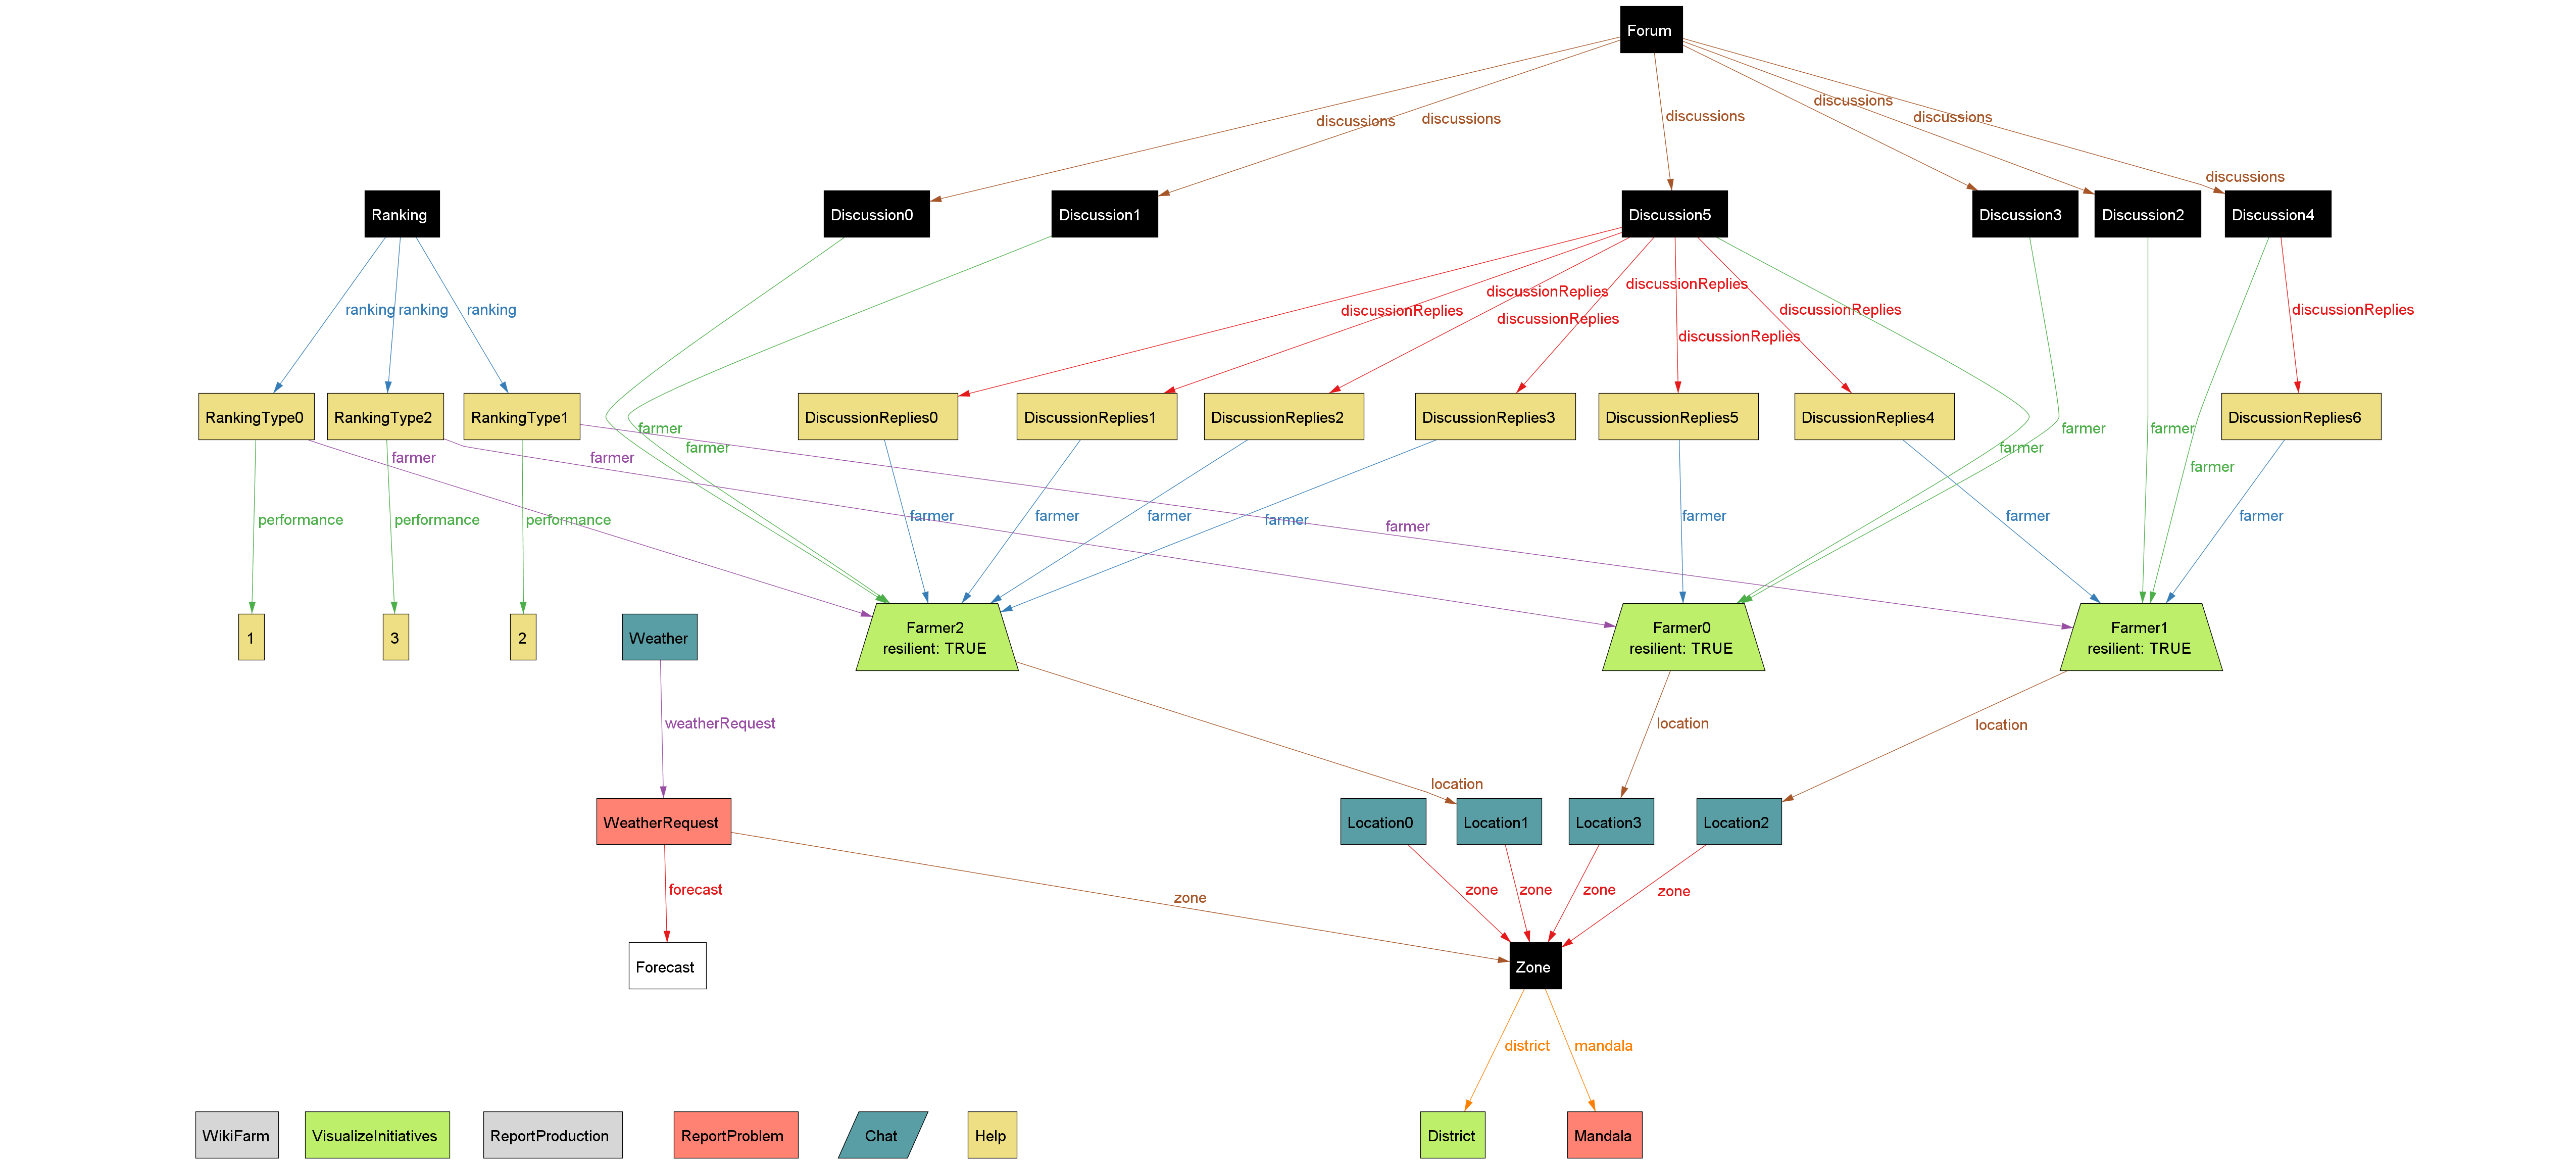
\includegraphics[angle=90,height=1.5\textwidth]{Images/Model/model3.png}
	\caption{Model of DIscussion}
\end{figure}

\subsection{WikiFarm and Visualize Initiatives}
This graph shows the WikiFarm functionality, which allows users to create requests based on their zone and type of production. It also shows the VisualizeInitiatives functionality, which allows TPM to visualize the reports produced by agronomists during their visits.\\
Below is presented the code used for generating the model.
\begin{lstlisting}
pred wikiFarm{
  #Seed = 0
  #Fertilizer = 0
  #TypeOfProduction = 3
  #DailyPlan = 2
  #DataProduction = 0
  #Forecast = 1
  #District = 1
  #Mandala >= #District
  #Zone = 2
  #Farmer = 3
  #TPM = 0
  #Agronomist = 1
  #HelpRequest = 0
  #Discussion = 0
  #DiscussionReplies = 0
  #Problem = 0
  #Messages = 0
  #Location = 3
  #WikiFarmRequest = 5
  #Report > 2
}
run wikiFarm for 15
\end{lstlisting}
\begin{figure}[H]
\centering
	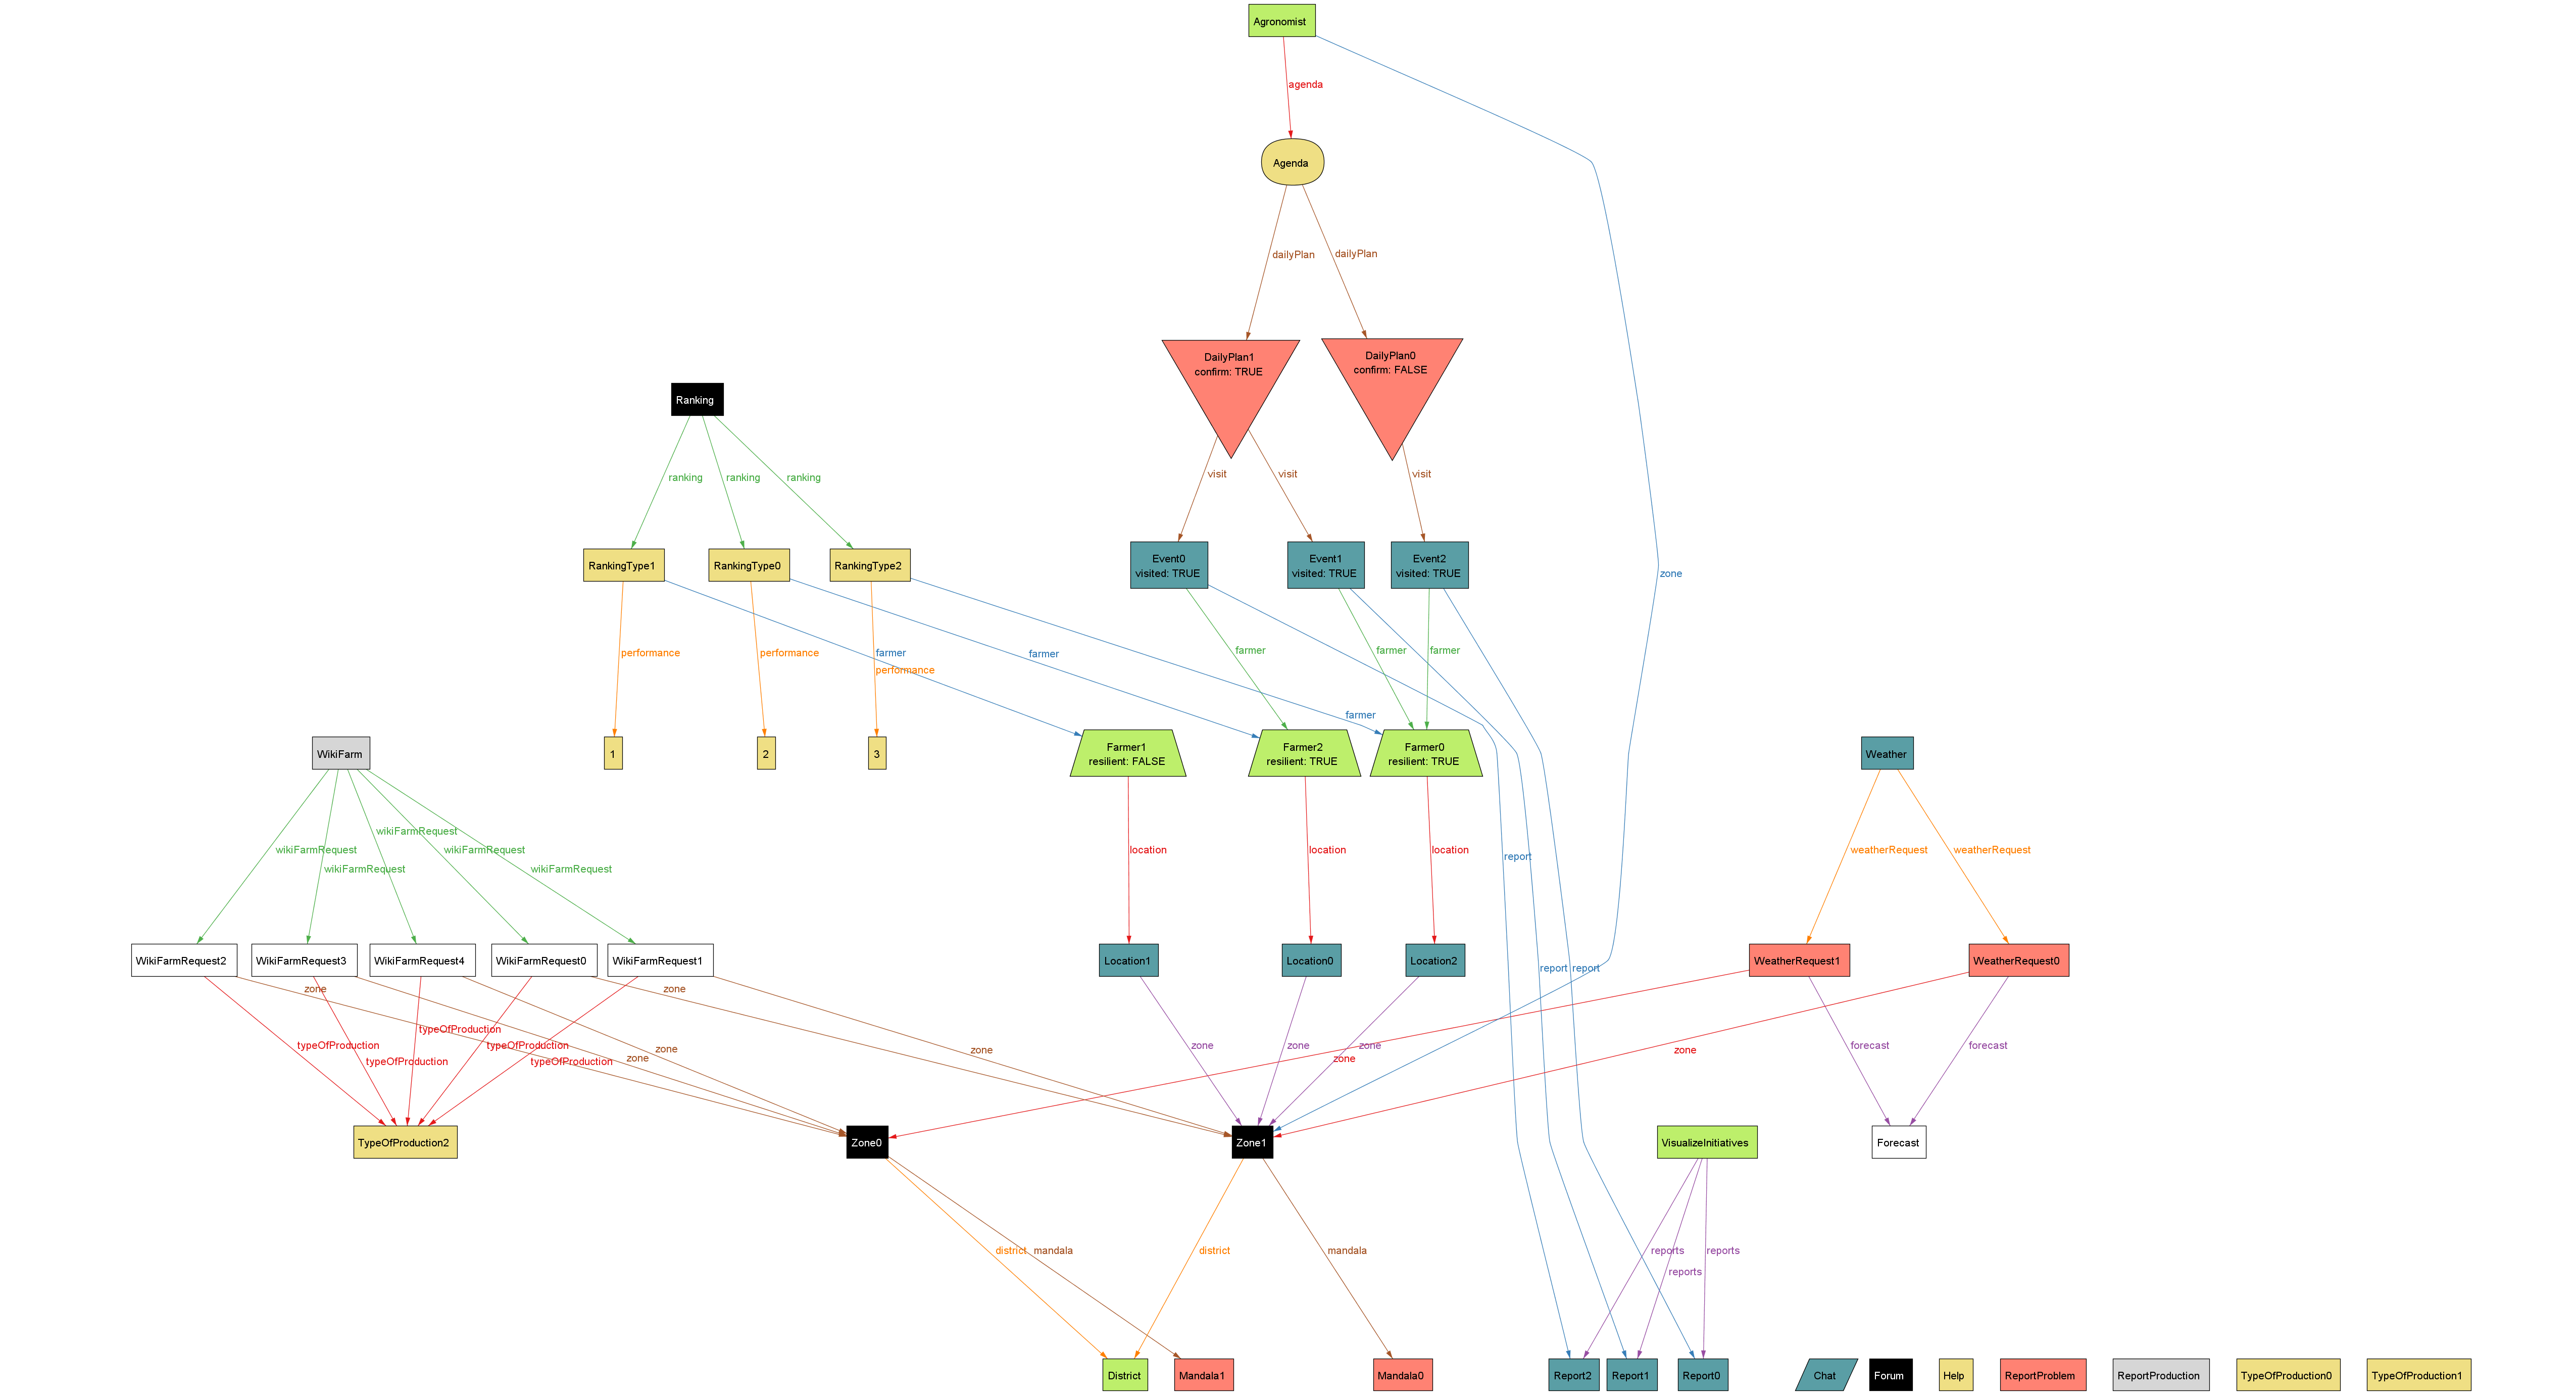
\includegraphics[angle=90,height=1.5\textwidth]{Images/Model/model4.png}
	\caption{Model of WikiFarm and Visualize Initiatives}
\end{figure}
